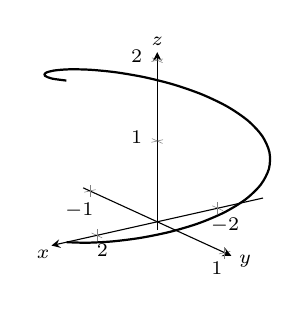
\begin{tikzpicture}[>=stealth]
\begin{axis}%
[width=175pt,tick label style={font=\scriptsize},axis on top,
			axis lines=center,
			view={145}{25},
			name=myplot,
			%xtick={1},
			%xlabel=$x$,ylabel=$y$,zlabel=$z$,
			%ytick=\empty,
			%ztick=\empty,
			ymin=-1.1,ymax=1.1,
			xmin=-3.5,xmax=3.5,
			zmin=-0.1, zmax=2.1,
			every axis x label/.style={at={(axis cs:\pgfkeysvalueof{/pgfplots/xmax},0,0)},xshift=-3pt,yshift=-3pt},
				xlabel={\scriptsize $x$},
			every axis y label/.style={at={(axis cs:0,\pgfkeysvalueof{/pgfplots/ymax},0)},xshift=5pt,yshift=-2pt},
				ylabel={\scriptsize $y$},
				every axis z label/.style={at={(axis cs:0,0,\pgfkeysvalueof{/pgfplots/zmax})},xshift=0pt,yshift=4pt},
				zlabel={\scriptsize $z$}
			]

\addplot3[domain=0:6.28,samples y=0,{\colorone},smooth,thick] ({3*cos(deg(x))},{sin(deg(x))},{x/3.14159});

%\addplot3 [no markers] coordinates {(0,0,0) (1,1,0)(0,2,0)(-1,1,0)(0,0,0)};

%\addplot3 [no markers] coordinates {(0,1,1) (1,2,1)(0,3,1)(-1,2,1)(0,1,1)};

%\filldraw [draw={\colorone},fill={\coloronefill},thick] (axis cs:0,1,1)--(axis cs:1,2,1)--(axis cs:0,3,1)--(axis cs:-1,2,1)--(axis cs:0,1,1);

%\filldraw [draw={\colorone},fill={\coloronefill},thick] (axis cs:0,1,1)--(axis cs:0,0,0)--(axis cs:1,1,0)--(axis cs:0,2,0)-- (axis cs:0,3,1) -- (axis cs:-1,2,1)--(axis cs:0,1,1);%--(axis cs:0,1,1);

%\draw [thick,{\colorone}] (axis cs: 0,1,1) -- (axis cs:1,2,1) -- (axis cs:0,3,1)  (axis cs:1,2,1) -- (axis cs:1,1,0);

%\draw[thick,{\colorone},dashed] (axis cs:0,0,0) -- (axis cs:-1,1,0) -- (axis cs:0,2,0)  (axis cs:-1,1,0) -- (axis cs:-1,2,1);

%\draw [very thick,black,->] (axis cs:0,0,0) -- (axis cs:1,1,0) node [left] {\scriptsize $\vec u$};
%\draw [very thick,black,->,dashed](axis cs:0,0,0) -- (axis cs:-1,1,0) node [above,pos=.7] {\scriptsize $\vec v$};
%\draw [very thick,black,->](axis cs:0,0,0) -- (axis cs:0,1,1) node [left,pos=.8] {\scriptsize $\vec w$};


%\addplot3[domain=-.1:1,y domain=-.1:1,surf,faceted color=black!20,samples=10,black!10] {-.1*x+y+1};
%
%\draw[>=stealth,->,thick] (axis cs:.1,.1,1.09) -- (axis cs: .7,.1,1.03) node [ left] {\scriptsize $\vec u$};
%
%\filldraw[black] (axis cs: .1,.1,1.09) circle (1pt);
%
%\draw[>=stealth,->,thick] (axis cs:.1,.1,1.09) -- (axis cs: .1,.8,1.79) node [right] {\scriptsize $\vec v$};
%

%
%\draw (axis cs: .5,.4,1.36) node  {\scriptsize $\theta$};

%\draw (axis cs: 0,0,\pgfkeysvalueof{/pgfplots/zmax}) node [shift={(0,0,20pt)}]{\scriptsize $z$};

%\draw (axis cs: 0,\pgfkeysvalueof{/pgfplots/ymax},0) node [shift={(0,2pt,0)}]{\scriptsize $y$};

%\draw (axis cs: \pgfkeysvalueof{/pgfplots/xmax},0,0) node [shift={(6pt,0,0)}]{\scriptsize $x$};

\end{axis}
%\node [right] at (myplot.right of origin)[shift={(-20pt,-8pt)}] {\scriptsize $y$};
%\node [above] at (myplot.above origin) [shift={(0,-5pt)}] {\scriptsize $z$};
\end{tikzpicture}









